\documentclass[11pt]{article}
\usepackage[margin=1in]{geometry}
\usepackage{amsmath,amssymb,booktabs,graphicx,hyperref,xcolor}
\usepackage[numbers]{natbib}
\usepackage[section]{placeins}
\hypersetup{colorlinks=true,linkcolor=black,citecolor=blue!50!black,urlcolor=blue!50!black}
\newcommand{\pending}[1]{\textcolor{red}{[#1]}}

\title{Bayes by Backprop's OOD Advantage Depends on Where Training Stops\\[4pt]
\large A softness-controlled study of mean-field VI along the optimization path}
\author{Saalik Mubeen\\Georgia Institute of Technology}
\date{October 2026}

\begin{document}
\maketitle

\begin{abstract}
Bayesian neural networks are often said to detect out-of-distribution (OOD)
inputs better than deterministic networks. But their predictions are softer
everywhere, and a deterministic network can be softened for free by a
temperature. I compare each method with a deterministic network softened to
the same in-distribution entropy, in a series of pre-registered experiments
on MLPs trained on MNIST. At typical training budgets, mean-field Bayes by
Backprop (BBB) is no better than this softness-matched network. Its advantage
($+0.06$ to $+0.08$ AUROC, more than a deep ensemble) appears only after
enough optimizer steps, and the number of steps, not the amount of data,
decides it. The posterior standard deviations grow along an almost identical
path for training sets of 500 to 10{,}000 images, suggesting that the
optimizer, not the data, sets the pace. Which uncertainty score is used then
matters. With predictive entropy the advantage can disappear later in
training, because the model also becomes uncertain on in-distribution inputs
as it underfits. With mutual information (MI) it persists, but MI also
``detects'' OOD inputs in runs that never learned the task. Neither held-out
NLL nor the ELBO selects a good stopping point, and a simple rule based on
synthetic outliers does no better than stopping at a fixed step. On CIFAR-10
with small, underfit models (37--68\% accuracy), no comparable advantage
appears.
\end{abstract}

\section{Introduction}
A standard classifier gives a confident prediction for any input, including
inputs unlike its training data. Bayesian neural networks (BNNs) average
predictions over a distribution of weights \citep{blundell2015weight}, which
should raise uncertainty on unfamiliar inputs. The usual evidence is that a
BNN's predictive entropy is higher on OOD data than a deterministic network's.

That evidence has a confound. A BNN's averaged prediction is softer than a
deterministic network's on every input, and temperature scaling
\citep{guo2017calibration} softens a deterministic network at no cost.
Temperature is a known ingredient of OOD detection \citep{liang2018enhancing}
and appears as a baseline in uncertainty benchmarks \citep{ovadia2019can}.
Whether BNNs are intrinsically good OOD detectors has been questioned
\citep{henning2021bayesian}, and a Bayesian last layer is known to reduce
overconfidence far from the data \citep{kristiadi2020being}. The comparison I
use throughout is simple: each method against a deterministic network
softened, on validation data only, to that method's own in-distribution
entropy. The question is whether the method ranks OOD inputs as more
uncertain than in-distribution inputs better than a network of the same
softness.

\paragraph{Findings.}
\begin{enumerate}
\item At standard training budgets, mean-field BBB is no better than the
softness-matched network on MNIST $\to$ Fashion-MNIST and KMNIST. Deep
ensembles are slightly better; MC dropout ties; last-layer Laplace is worse
(\S\ref{sec:grid}).
\item BBB's advantage is set by the number of optimizer steps, not by the
training-set size (\S\ref{sec:steps}). The posterior standard deviations
follow nearly the same trajectory at every $n$ (\S\ref{sec:clock}).
\item Along training, the entropy-based advantage can rise and fall while the
MI-based advantage persists; MI is also high for models that never learned
(\S\ref{sec:window}).
\item The advantage needs posterior noise in both hidden layers together, and
it is not a pixel shortcut (\S\ref{sec:mechanism}).
\item Neither held-out NLL nor the ELBO picks a good stopping point. A
synthetic-outlier rule does no better than a fixed step count
(\S\ref{sec:select}).
\item On CIFAR-10 with small, underfit models, no comparable advantage
appears (\S\ref{sec:cifar}).
\end{enumerate}
Every experiment had its hypothesis, predictions and falsification criteria
committed to git before it ran. Appendix~\ref{app:ledger} lists all
predictions, including the many that failed.

\section{Setup}\label{sec:setup}
\paragraph{Data.} MNIST training subsets of $n\in\{500, 2{,}000, 10{,}000\}$
class-stratified images (one per seed); a fixed validation pool of 5{,}000
further training images, disjoint from every subset; the MNIST test set; OOD:
Fashion-MNIST \citep{xiao2017fashion} and KMNIST \citep{clanuwat2018deep} test
sets, normalised with MNIST statistics. CIFAR-10 experiments are described in
\S\ref{sec:cifar}.

\paragraph{Models.} All MNIST models use a 784--256--256--10 ReLU MLP.
\emph{DNN}: Adam ($10^{-3}$, cosine), 40 epochs, batch 64. \emph{MAP}: the
same network trained to the MAP estimate under BBB's $\mathcal N(0,1)$ prior,
with BBB's budget (150 epochs, gradient clipping). \emph{MC dropout}
\citep{gal2016dropout}: $p=0.1$, 50 samples. \emph{Deep ensemble}
\citep{lakshminarayanan2017simple}: 5 DNNs. \emph{Last-layer Laplace}
\citep{daxberger2021laplace}: full generalised Gauss--Newton covariance over
the last layer of a DNN, prior precision tuned on validation NLL. \emph{BBB}
\citep{blundell2015weight}: mean-field Gaussian posterior, $\mathcal N(0,1)$
prior, per-example negative ELBO
\begin{equation}
\mathcal{L} = \frac{1}{B}\sum_{i\in\text{batch}} -\log p(y_i\mid x_i, w)
+ \frac{1}{N}\,\mathrm{KL}\big[q(w)\,\|\,p(w)\big], \qquad w=\mu+\sigma\odot\varepsilon,
\label{eq:elbo}
\end{equation}
with the KL weight warmed up linearly, $\sigma=\mathrm{softplus}(\rho)$ and
$\rho$ initialised at $-5$ ($\sigma_0\approx 0.007$), Adam $10^{-3}$, gradient
clipping, 50 posterior samples at test time. By default BBB trains for 150
epochs at $n\ge 2{,}000$ (4{,}800 steps at $n=2{,}000$) and the same number of
steps at $n=500$.

\paragraph{The softness-matched control.} For a method $M$, I fit a
temperature $T$ to a DNN's logits so that its mean predictive entropy on the
\emph{validation} set equals $M$'s. No test or OOD data enters the fit. The
reported quantity is
$\Delta = \mathrm{AUROC}(M) - \mathrm{AUROC}(\mathrm{DNN}_T)$, where AUROC
measures the separation of test from OOD images by predictive entropy.
$\Delta>0$ means $M$ ranks OOD inputs better than a network of the same
softness. I report both entropy- and MI-based AUROC where relevant.
Comparisons are paired by seed, with bootstrap confidence intervals and sign
counts (wins out of seeds). Wilcoxon tests are reported only with 10 seeds,
since with 5 seeds they cannot fall below $p=0.0625$. Unless stated otherwise,
BBB predictions use 50 posterior samples. The training-dynamics runs
(\S\ref{sec:window}, \S\ref{sec:select}) use 20, which slightly
under-estimates OOD entropy, so their $\Delta$ values are conservative.

\section{Results on MNIST}

\subsection{At standard budgets, only ensembles beat the control}\label{sec:grid}
Table~\ref{tab:grid} compares each method with its own softness-matched DNN
over 10 seeds. At $n=500$ and $2{,}000$, BBB is significantly \emph{worse}
than the control; at $n=10{,}000$ it is much better, in all 10 seeds.
\S\ref{sec:steps} shows that this jump is not about data. Deep ensembles beat
the control at every $n$ by $+0.01$ to $+0.02$; against a stronger,
budget-matched MAP network their edge mostly disappears at $n=2{,}000$. MC
dropout roughly ties the control, and last-layer Laplace is clearly below it.

\begin{table}[!htb]
\centering\small
\begin{tabular}{llcc}
\toprule
$n$ & method & $\Delta$ Fashion [95\% CI] & $\Delta$ KMNIST [95\% CI] \\
\midrule
500 & BBB & $-0.046$ [$-0.063$, $-0.032$] & $-0.035$ [$-0.041$, $-0.028$] \\
500 & ensemble & $+0.014$ [$0.003$, $0.027$] & $+0.010$ [$0.008$, $0.012$] \\
500 & MC dropout & $-0.003$ [$-0.016$, $0.009$] & $-0.019$ [$-0.021$, $-0.018$] \\
500 & last-layer Laplace & $-0.072$ [$-0.088$, $-0.055$] & $-0.112$ [$-0.122$, $-0.102$] \\
\midrule
2{,}000 & BBB & $-0.024$ [$-0.048$, $-0.001$] & $-0.010$ [$-0.014$, $-0.007$] \\
2{,}000 & ensemble & $+0.015$ [$0.007$, $0.022$] & $+0.015$ [$0.013$, $0.018$] \\
2{,}000 & MC dropout & $+0.007$ [$0.002$, $0.012$] & $-0.010$ [$-0.012$, $-0.007$] \\
2{,}000 & last-layer Laplace & $-0.040$ [$-0.047$, $-0.032$] & $-0.043$ [$-0.047$, $-0.038$] \\
\midrule
10{,}000 & BBB & $\mathbf{+0.048}$ [$0.038$, $0.059$] & $\mathbf{+0.069}$ [$0.065$, $0.074$] \\
10{,}000 & ensemble & $+0.016$ [$0.008$, $0.026$] & $+0.023$ [$0.021$, $0.025$] \\
10{,}000 & MC dropout & $-0.010$ [$-0.018$, $-0.001$] & $-0.007$ [$-0.010$, $-0.003$] \\
10{,}000 & last-layer Laplace & $-0.014$ [$-0.023$, $-0.006$] & $-0.012$ [$-0.016$, $-0.008$] \\
\bottomrule
\end{tabular}
\caption{Each method vs a DNN softened to its own validation entropy (entropy
AUROC difference, 10 seeds). Source: \texttt{experiments/E2\_mnist\_grid}.}
\label{tab:grid}
\end{table}

On accuracy, BBB beats the budget-matched MAP network by 1.1 points at
$n=500$ and 0.5 points at $n=2{,}000$ (9/10 and 10/10 seeds), and loses by 0.5
points at $n=10{,}000$. About half of its apparent lead over the plain DNN at
$n=2{,}000$ is ordinary regularisation.

\subsection{The advantage follows optimizer steps, not data}\label{sec:steps}
With fixed epochs, a larger $n$ also means more optimizer steps: 23{,}550 at
$n=10{,}000$ vs 4{,}800 at $n\le 2{,}000$. Figure~\ref{fig:steps} decouples
the two. With the same data, 23{,}550 steps give $\Delta=+0.06$ to $+0.08$ in
5/5 seeds at every $n$, including $n=500$. 4{,}800 steps give no advantage,
including at $n=10{,}000$. Over this range the training-set size barely
matters.

\begin{figure}[!htb]
\centering
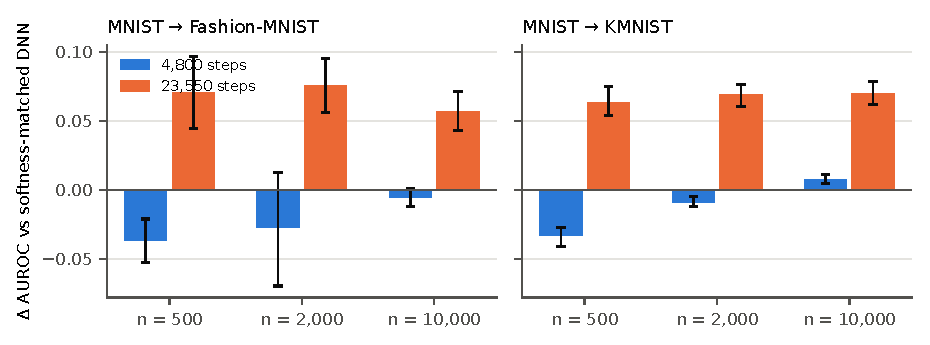
\includegraphics[width=0.92\linewidth]{../figures/paper_steps_vs_n.pdf}
\caption{BBB vs its softness-matched DNN with the same training data and two
step budgets (5 seeds, 95\% CIs). Source: \texttt{experiments/E4\_steps\_vs\_n}.}
\label{fig:steps}
\end{figure}

\subsection{Along training: entropy and MI diverge}\label{sec:window}
To see what happens in between, I trained BBB for 50{,}000 steps at
$n=2{,}000$ with a \emph{constant} learning rate and evaluated every 1{,}000
steps (Figure~\ref{fig:dyn}). With the default initialisation, the
entropy-based $\Delta$ on KMNIST is negative for the first $\sim$3{,}000 steps,
peaks at $+0.067$ to $+0.074$ around 9{,}000--14{,}000 steps (mean
first-layer $\sigma$ 0.65--0.82), and is negative again at 25{,}000--30{,}000
steps. The MI-based $\Delta$ does not fall: it is $+0.073$ at 10{,}000 steps,
$+0.071$ at 30{,}000 and $+0.061$ at 50{,}000. The entropy advantage disappears
because the model also becomes uncertain on in-distribution digits. Mean test
entropy rises from 0.30 to 0.94 as accuracy falls from 0.93 to 0.89. The
negative ELBO keeps improving throughout (143 at 4{,}000--5{,}000 steps, 6.8 at
24{,}000--25{,}000, 3.5 at 50{,}000). It drifts towards a posterior with
$\sigma\approx 0.98$ in the hidden layers (0.93 in the last), accuracy 0.89
and ECE 0.19. That is consistent with Coker et al.'s analysis of wide
mean-field BNNs \citep{coker2022wide}, whose theorem covers a different
setting (regression, odd activations). The entropy collapse is specific to
$n=2{,}000$: at 40{,}000 steps the entropy-based $\Delta$ is still $+0.033$
($n=500$) and $+0.060$ ($n=10{,}000$) on KMNIST.

Two cautions about MI. First, a slightly larger initial $\sigma$ (0.049)
reaches the advantage sooner (3{,}000 steps instead of 6{,}000), but
initialising $\sigma\ge 0.31$ prevents learning altogether: accuracy stays at
chance in a local optimum with a far worse ELBO (9.0--9.2 vs 3.4--3.5). These
chance-level models have the \emph{largest} MI-based $\Delta$ (about $+0.10$).
A positive MI $\Delta$ therefore does not by itself show a useful model. It
also reflects disagreement between near-prior posterior samples on any unusual
input. Second, these runs use a constant learning rate; the E4 runs
(\S\ref{sec:steps}) used a cosine schedule, which freezes training wherever the
budget ends.

\begin{figure}[!htb]
\centering
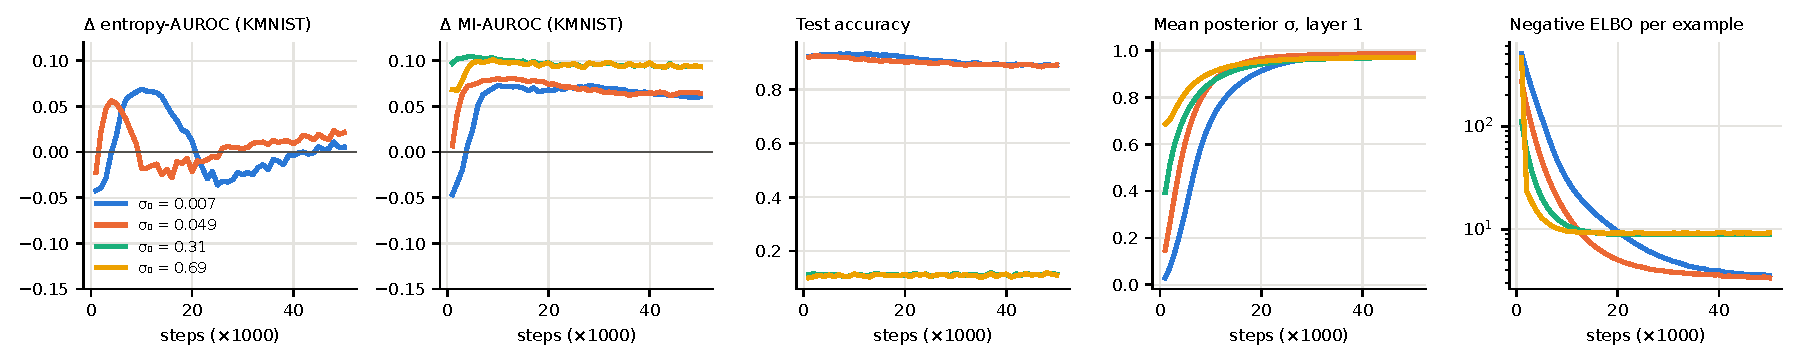
\includegraphics[width=\linewidth]{../figures/E6_dynamics.pdf}
\caption{BBB training dynamics at $n=2{,}000$ (constant learning rate; mean of
3 seeds per initial $\sigma_0$; 20 posterior samples). Runs with
$\sigma_0\ge 0.31$ never learn; their entropy-based $\Delta$ (about $-0.86$) is
below the plotted range. Source: \texttt{experiments/E6\_dynamics}.}
\label{fig:dyn}
\end{figure}

\subsection{An optimizer clock}\label{sec:clock}
Why do steps matter more than data? In the E9 runs (constant learning rate
$10^{-3}$, $\rho_0=-5$), the mean first-layer $\rho$ (with
$\sigma=\mathrm{softplus}(\rho)$) follows nearly the same path at every
training-set size. It is $-3.54$, $-3.52$ and $-3.62$ after 1{,}000 steps,
$-1.88$, $-1.85$ and $-1.92$ after 3{,}000, and $-1.01$, $-0.99$ and $-1.09$
after 5{,}000, for $n = 500$, $2{,}000$ and $10{,}000$. With $\sigma$ tiny at
initialisation, the gradient on $\rho$ is dominated by the KL term. Adam
normalises its updates, so each step moves $\rho$ by roughly the learning rate
whatever the KL weight $1/N$ is. Unlu and Aitchison
\citep{unlu2020variational} point out this step bound for mean-field
variances. If this explanation is right, BBB's state, and hence its OOD
behaviour, is set by the learning rate times the number of steps and the
initial $\sigma$, not by $N$. I have not yet tested this directly (by varying
the learning rate, or by replacing Adam with SGD, where $1/N$ should matter),
so it is a hypothesis.

\subsection{What produces the advantage}\label{sec:mechanism}
\paragraph{Noise in both hidden layers.} Taking BBB models trained for 23{,}550 steps,
I switched posterior noise off layer by layer. Noise in the first and second
layers together keeps 73--82\% of $\Delta$. Noise in any single layer keeps
essentially none (first layer: 16\% on Fashion-MNIST, $-26\%$ on KMNIST).
The posterior-mean network on its own is a worse OOD detector than the DNN.
The advantage comes from noise compounding across the hidden layers, which a
last-layer method cannot produce.

\paragraph{Not a pixel shortcut.} Many pixels are constant (always
background) across a training subset: on average 192, 148 and 104 at
$n=500$, $2{,}000$ and $10{,}000$. A model-free rule, ``flag
any image with ink on such a pixel'', separates MNIST from Fashion-MNIST and
KMNIST with AUROC 0.967--1.000 over 15 training subsets (means
0.990--1.000), a real weakness of these benchmarks. But the
models do not rely on it. Resetting those pixels to background in the OOD
images leaves every method's AUROC and $\Delta$ essentially unchanged (BBB at
$n=10{,}000$: $+0.057\to+0.055$ and $+0.070\to+0.070$). The growth of
$\sigma$ is also global, not concentrated on those pixels (ratio 1.0--1.24).

\subsection{Choosing when to stop}\label{sec:select}
Neither in-distribution criterion picks a good checkpoint. Minimum held-out
NLL stops at 1{,}000--3{,}000 steps, before the advantage appears; minimum
$-$ELBO stops at the end of training. I tested a rule that needs no real OOD
data. I built three synthetic outlier sets from the validation images
(uniform noise, flipped digits, pixel-permuted digits) and picked the
checkpoint that best separates validation images from them by MI
(Table~\ref{tab:select}; 12 runs, $n\in\{500, 2{,}000, 10{,}000\}$). It reaches
73\% of the best achievable entropy-based advantage (the ``oracle''), but
simply stopping at a fixed 8{,}000 steps reaches 72\%. Scoring the last
checkpoint by MI instead of entropy, with no selection at all, does as well
($+0.049$). The oracle is a maximum over 40 checkpoints and is optimistic. These
runs also share configurations and seeds with \S\ref{sec:window}. The proxy
rule therefore does not beat trivial alternatives here.

\begin{table}[!htb]
\centering\small
\begin{tabular}{lccc}
\toprule
rule & mean step & $\bar\Delta$ (entropy) & fraction of oracle \\
\midrule
oracle (uses real OOD; optimistic) & 10{,}917 & $+0.067$ & 1.00 \\
synthetic-outlier proxies (MI) & 10{,}417 & $+0.049$ & 0.73 \\
fixed stop at 8{,}000 steps & 8{,}000 & $+0.048$ & 0.72 \\
fixed stop at 10{,}000 steps & 10{,}000 & $+0.047$ & 0.71 \\
minimum $-$ELBO & 39{,}417 & $+0.034$ & 0.52 \\
minimum validation NLL & 2{,}250 & $-0.032$ & $-0.49$ \\
\bottomrule
\end{tabular}
\caption{Stopping rules ($\bar\Delta$ = mean of Fashion-MNIST and KMNIST
entropy-based $\Delta$ at the chosen checkpoint; 12 runs). Source:
\texttt{experiments/E9\_selection}, \texttt{results/E9/}.}
\label{tab:select}
\end{table}

\section{CIFAR-10}\label{sec:cifar}
I repeated the dynamics experiment on CIFAR-10 ($n=10{,}000$, no
augmentation) with a small CNN (three $3\times3$ conv layers of 32, 64 and
128 channels, then 256 and 10 units), every layer Bayesian. OOD sets were SVHN
(10{,}000 images) and CIFAR-100. No comparable advantage appeared (Figure~\ref{fig:cifar}).
BBB's peak $\Delta$ on SVHN was $-0.044$, $+0.006$ and $-0.056$ in the three
seeds, and on CIFAR-100 at most $+0.031$, early in training. Even a 5-member
deep ensemble lost to a single softness-matched DNN on SVHN (AUROC
0.727--0.740 vs 0.759--0.807), while winning on CIFAR-100 by $+0.02$ to $+0.03$.
Scored by MI instead, BBB was \emph{worse} on SVHN: MI-AUROC ranged from 0.24
to 0.60 across checkpoints, often below chance. The drift towards the prior
did replicate. The large fully connected layer's
$\sigma$ reached 0.996, the ELBO kept improving, and accuracy fell from
0.67--0.68 to 0.61--0.63. The first conv layer's $\sigma$ stayed small (0.04).

To separate architecture from data, I trained the MNIST study's MLP on
flattened CIFAR-10 images at $n=2{,}000$ and $10{,}000$ (3 seeds each). Its
deterministic version reaches 38\% and 46\% test accuracy. BBB again showed no
advantage on SVHN (peak $\Delta$ $-0.031$ to $+0.030$). On CIFAR-100 it gained
$+0.030$ to $+0.046$ for the first few thousand steps, similar to the CNN's
$+0.024$ to $+0.031$. Then it collapsed towards the prior (first-layer
$\sigma\to0.997$--$0.999$, accuracy falling to 0.10--0.29). Much larger
CIFAR-100 ``gains'' at $n=2{,}000$ ($+0.09$ to $+0.21$) appear only after
collapse, at near-chance accuracy, and are not meaningful. My pre-registered
decision rule counted these runs as support for an architectural
explanation, but it had no accuracy condition, and the qualifying gains are
barely above its threshold and no larger than the CNN's. On natural images,
neither architecture shows the MNIST-sized advantage ($+0.06$ to $+0.08$ on both
OOD sets). The evidence points more to the data, or to the much harder task
(37--47\% accuracy), than to the CNN's structure.

\begin{figure}[!htb]
\centering
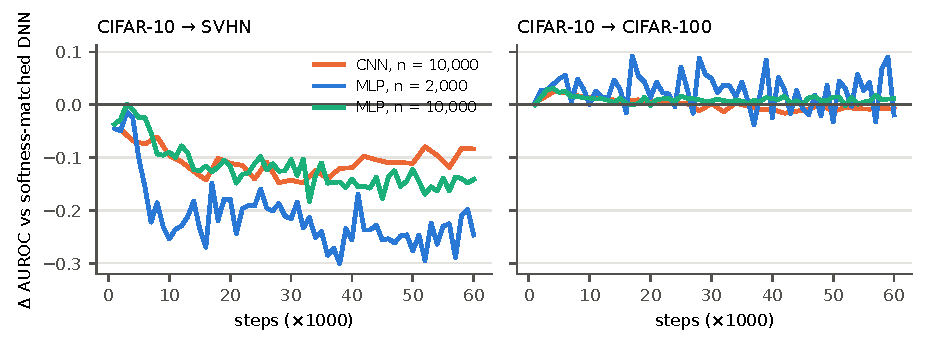
\includegraphics[width=0.92\linewidth]{../figures/paper_cifar.pdf}
\caption{BBB vs its softness-matched network on CIFAR-10 over training (mean
of 3 seeds per curve; CNN from all layers Bayesian, MLP = the MNIST
architecture on flattened images). Sources: \texttt{experiments/E7\_cifar},
\texttt{experiments/E7b\_cifar\_mlp}.}
\label{fig:cifar}
\end{figure}

\section{Related work}
Coker et al.\ \citep{coker2022wide} prove that the optimal mean-field
posterior predictive approaches the prior predictive as width grows; the drift
in \S\ref{sec:window} is consistent with that effect along the optimisation
path of a standard-width ReLU classifier, a setting their theorem does not cover. Unlu and Aitchison \citep{unlu2020variational} note
that mean-field variances are often unconverged when training stops; here
that state is exactly where BBB looks like a tempered DNN. Izmailov et al.\
\citep{izmailov2021dangers} show that weights on always-zero pixels keep their
prior under HMC and hurt accuracy under covariate shift; I find no such
pixel-specific effect in BBB's OOD detection. Ovadia et al.\
\citep{ovadia2019can} include temperature-scaled baselines and find ensembles
strongest under shift. Odgers et al.\ \citep{odgers2026gaussian} show that mean-field VI can
overestimate predictive variance on in-distribution points, which matches the
rising in-distribution entropy in \S\ref{sec:window}. Trippe and Turner
\citep{trippe2018overpruning} describe overpruning, where variational BNNs
switch off units by sending their weights to the prior. Fortuin et al.\
\citep{fortuin2022priors} show that isotropic Gaussian priors are often poor
choices for neural networks. Henning et al.\ \citep{henning2021bayesian} question
whether exact BNN posteriors are intrinsically good OOD detectors. Raina and
Schmah \citep{raina2025ood} report Bayesian advantages for OOD detection from
small training sets; the results here suggest checking training length and
softness before attributing such advantages to the posterior.

\section{Limitations}
\begin{itemize}
\item \textbf{Scope.} The positive results come from small MLPs on
MNIST-family data. The CIFAR-10 models were small and underfit (37--68\%
accuracy, no augmentation), so the CIFAR result says little about well-trained
networks.
\item \textbf{Prior.} The $\mathcal N(0,1)$ prior is badly misspecified for
layers whose weights have scale $\sim0.05$ \citep{fortuin2022priors}, so a
drift towards it is expected to hurt fit. I have not swept the prior scale.
\item \textbf{Schedule and samples.} The dynamics runs use a constant learning
rate and 20 posterior samples; the fixed-budget runs use a cosine schedule and
50 samples.
\item \textbf{Statistics.} Dynamics results rest on 3 seeds per setting, and the
selection analysis reuses those configurations and seeds.
\item \textbf{No exact posterior.} Without HMC or similar, I cannot say whether
any of this reflects Bayesian behaviour or only mean-field VI under Adam.
\end{itemize}

\section{Conclusion}
For Bayes by Backprop on MNIST-family data, ``knowing what it doesn't know''
is not a fixed property of the method. It depends on how many optimizer steps
were taken and on which uncertainty score is reported. At typical budgets BBB
behaves like a temperature-scaled network. With longer training its
mutual-information signal separates OOD inputs well, but the same signal
appears in models that never learned, and entropy-based scores can lose the
advantage as the model underfits. Comparisons between BBB and deterministic
or ensemble methods should report the training budget, the score and a
softness-matched baseline.

\paragraph{Reproducibility.} Code: \texttt{bnnstudy/}; every command:
\texttt{COMMANDS.md}; every number in this report: \texttt{CLAIMS.md};
pre-registered protocols with results: \texttt{experiments/}.

\appendix
\section{KL scaling}\label{app:kl}
Dividing the KL term in Eq.~\ref{eq:elbo} by the number of mini-batches
instead of by $N$ is an easy slip when the cross-entropy is averaged per
batch. It over-weights the KL term by $N/\lceil N/B\rceil\approx B$ (62.5$\times$
at $N=2{,}000$, $B=64$). In a 3-seed pilot it cost BBB 3.2 points of accuracy
(0.904 vs 0.936) and raised ECE from 0.022 to 0.185.

\section{Pre-registered predictions and outcomes}\label{app:ledger}
Each protocol (\texttt{experiments/<id>/protocol.md}) was committed before its
runs. Of the 29 entries below, 9 were confirmed, 16 falsified, 3 had mixed
outcomes and 1 had no outcome. (E5's P1 held by construction and is omitted.) The falsified ones are what moved the study from ``is the advantage
just softness?'' to the training-path account.

\begin{center}\small
\begin{tabular}{p{0.9cm}p{8.6cm}p{4.6cm}}
\toprule
exp. & prediction & outcome \\
\midrule
E1 & P0: new pipeline reproduces old numbers ($\pm0.02$ acc, $\pm0.03$ AUROC) & acc/ECE yes; AUROC off by 0.035 \\
E1 & P1: correct KL weight raises BBB accuracy & confirmed \\
E1 & P2: BBB within 0.02 AUROC of softness-matched DNN & falsified (Fashion) \\
E2 & P1: BBB never beats the control & falsified ($n=10{,}000$) \\
E2 & P2: ensembles beat the control & confirmed \\
E2 & P3: MC dropout and Laplace within 0.02 of the control & dropout yes; Laplace falsified \\
E2 & P4: larger KL weight lowers accuracy, raises KMNIST MI-AUROC & confirmed \\
E3 & P1: BBB and budget-matched MAP equally accurate ($<0.005$) & falsified (narrowly) \\
E3 & P2: BBB never beats softness-matched MAP & falsified ($n=10{,}000$) \\
E4 & P1: the gain follows optimizer steps, not $n$ & confirmed \\
E4 & P2: dead-pixel weights have $>5\times$ the $\sigma$ of live ones & falsified \\
E4 & P3: $n=500$ with long training shows the gain & confirmed \\
E5 & P2: removing dead-pixel ink halves BBB's gain & falsified \\
E5 & P3: removing it shrinks the ensemble's gain & falsified \\
E5 & P4: the DNN's AUROC drops less than BBB's when the ink is removed & falsified (neither drops) \\
E6 & P1: $\Delta$ rises with $\sigma$ & falsified (peaks, then falls) \\
E6 & P2: $\Delta$ plateaus & falsified (transient) \\
E6 & P3: larger $\sigma_0$ reaches the gain sooner & falsified ($\sigma_0\ge0.31$ never learns) \\
E6 & P4: ELBO still improving at 4{,}800 steps & confirmed \\
E6b & P1: first-layer noise alone keeps $\ge70\%$ & falsified \\
E6b & P2: last-layer noise alone keeps $<30\%$ & confirmed \\
E9 & P1: combined proxies reach $\ge70\%$ of oracle; NLL $\le20\%$ & confirmed, but a fixed 8k-step stop does as well \\
E9 & P2: one proxy alone reaches $\ge70\%$ & falsified (67\%) \\
E9 & P3: peak step rises with $n$ & confirmed by mean; not robust \\
E7 & P1: window on SVHN with a CNN & falsified \\
E7 & P2: window closes & no outcome (no window) \\
E7 & P3: proxy selection beats NLL & falsified \\
E7 & P4: ensemble beats the control on SVHN & falsified \\
E7b & rule: architecture vs data & ``architecture'' by the rule; weak \\
\bottomrule
\end{tabular}
\end{center}

\bibliographystyle{unsrtnat}
\bibliography{refs}
\end{document}
